
\section{Introduction}

\begin{frame}{Genetic Algorithms using Neural Networks}

  \begin{itemize}
    \item Population with individuals
    \item Individuals are candidate solutions
    \item Neural networks as candidate solutions
  \end{itemize}
  \begin{itemize}
    \item Motivation?
    \item Measuring diversity?
  \end{itemize}
%  introduction of some sort
%  what did we work with (briefly)
%  why did we do it? (motivation)
%  how did we end up working with diversity?
\end{frame}

\begin{frame}{Fun and exciting}
  \begin{figure}
    \centering
    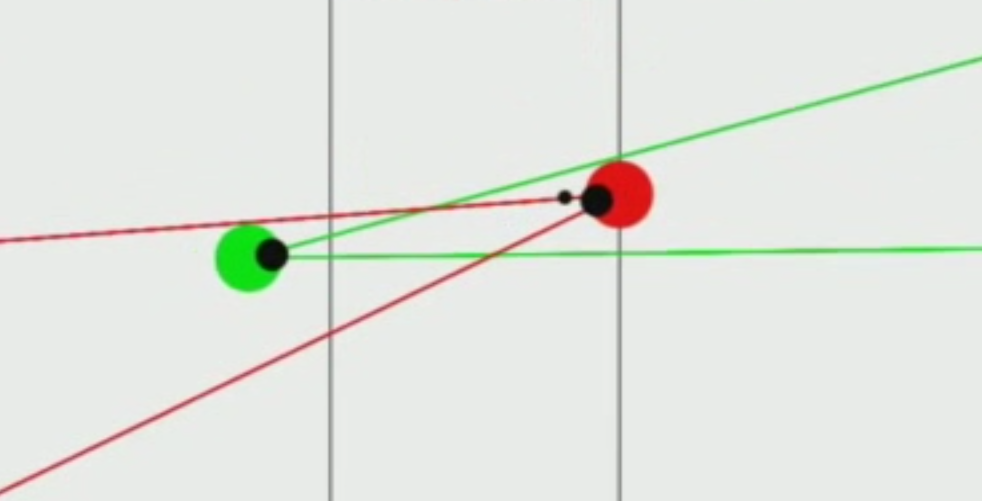
\includegraphics[width=250px]{elias/images/sniper.png}
    \caption{\url{youtube.com/watch?v=u2t77mQmJiY}}
    %by Ding Nicolas
  \end{figure}
\end{frame}

%\begin{frame}{Motivation}
%  \begin{figure}
%    \centering
%    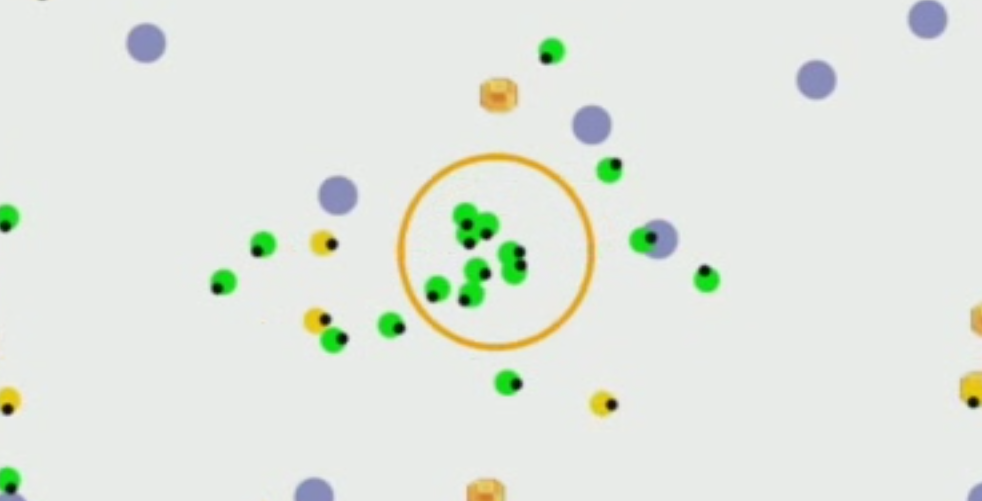
\includegraphics[width=250px]{elias/images/swarm.png}
%    \caption{\url{youtube.com/watch?v=Iv_Fy6Urik4}}
    %by Ding Nicolas
%  \end{figure}
%\end{frame}

\begin{frame}{Useful and serious}
  \begin{figure}
    \centering
    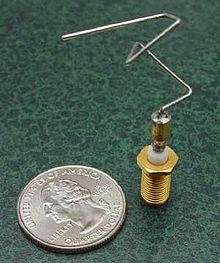
\includegraphics[height=100px]{elias/images/antenna.jpg}
    \caption{\url{en.wikipedia.org/wiki/genetic_algorithm}}
  \end{figure}
\end{frame}

%\section{Candidate Solutions}

\begin{frame}{Structuring Candidate Solutions}
  \begin{center}
    \scalebox{0.8}{
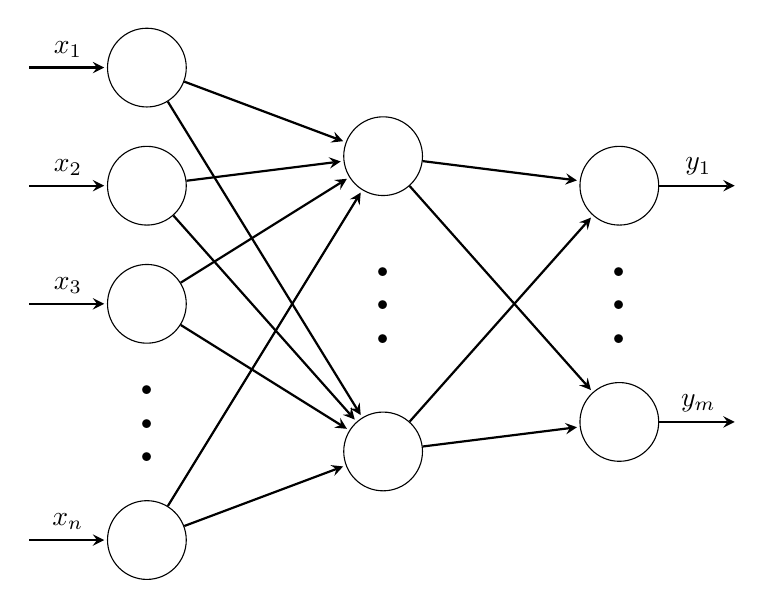
\begin{tikzpicture}
  [x=1.5cm, y=1.5cm, >=stealth, shorten >=1pt,
    every neuron/.style={
      circle,
      draw,
      minimum size=1cm
    },
    neuron missing/.style={
      draw=none, 
      scale=3,
      text height=0.333cm,
      execute at begin node=\color{black}$\vdots$
    },
  ]
% Draw input nodes
\foreach \m/\l [count=\y] in {1,2,3,missing,4}
  \node [every neuron/.try, neuron \m/.try] (input-\m) at (0,2.5-\y) {};

% Label input edges 
\foreach \l [count=\i] in {1,2,3,n}
  \draw [<-, shorten <=1pt, shorten >=0pt,thick] (input-\i) -- ++(-1,0)
  node [above, midway] {$x_\l$};

% Draw hidden nodes
\foreach \m [count=\y] in {1,missing,2}
  \node [every neuron/.try, neuron \m/.try ] (hidden-\m) at (2,2-\y*1.25) {};

% Draw output nodes
\foreach \m [count=\y] in {1,missing,2}
  \node [every neuron/.try, neuron \m/.try ] (output-\m) at (4,1.5-\y) {};

% Label output edges 
\foreach \l [count=\i] in {1,m}
  \draw [->,thick] (output-\i) -- ++(1,0)
  node [above, midway] {$y_\l$};

% Connect input nodes with hidden nodes
\foreach \i in {1,...,4}
  \foreach \j in {1,...,2}
    \draw [->,thick] (input-\i) -- (hidden-\j);

% Connect hidden nodes with output nodes
\foreach \i in {1,...,2}
  \foreach \j in {1,...,2}
    \draw [->,thick] (hidden-\i) -- (output-\j);
\end{tikzpicture}}

  \end{center}
%  picture of use of neural networks
\end{frame}

\begin{frame}{Representing Candidate Solutions}
  \begin{itemize}
    \item Static network structure
    \item Weights represent the network as bit strings
    \item Straightforward manipulation
  \end{itemize}
%  bit strings as chromosomes to be manipulated
\end{frame}

\begin{frame}{Assessing Candidate Solutions}
  \begin{itemize}
    \item How good is a candidate solution? How fit is it?
    \item Which conditions are important to observe?
    \item Defining a fitness function
  \end{itemize}
%  fitness functions and importance
\end{frame}

\section{Existing Diversity Measures}

\begin{frame}{Existing Diversity Measures}
  \begin{itemize}
    \item Genotypic diversity measure (genetic make-up)
    \item Phenotypic diversity measure (behaviour/fitness)
  \end{itemize}
\end{frame}

\begin{frame}{Genotypic measures}
  \begin{figure*}
  \begin{subfigure}{0.5\textwidth}
    \centering
    \inputresizeto{0.5\linewidth}{drawings/eqnetworks/eqnetworks3}
    \caption{An artificial neural network with connections and weights.}\label{fig:eqnetwork}
  \end{subfigure}
  \begin{subfigure}{0.5\textwidth}
    \centering
    \inputresizeto{0.5\linewidth}{drawings/eqnetworks/eqnetworks4}
    \caption{An artificial neural network equivalent to \cref{fig:eqnetwork}.}\label{fig:eqnetwork2}
  \end{subfigure}
  \caption{Networks with same phenotype, but different genotypes. The binary representation assumes that each weight is represented by four bits.}\label{fig:entire-eqnetwork}
\end{figure*}


  \begin{itemize}
    \item Hamming distance of 6
    \item Levenschtein distance of 6
    \item Genotypically diverse
    \item Always produce the same output
  \end{itemize}
%  illustration of the workings of hamming distance
\end{frame}

\begin{frame}{Fitness-based phenotypic measure}
  \begin{figure}
    \centering
    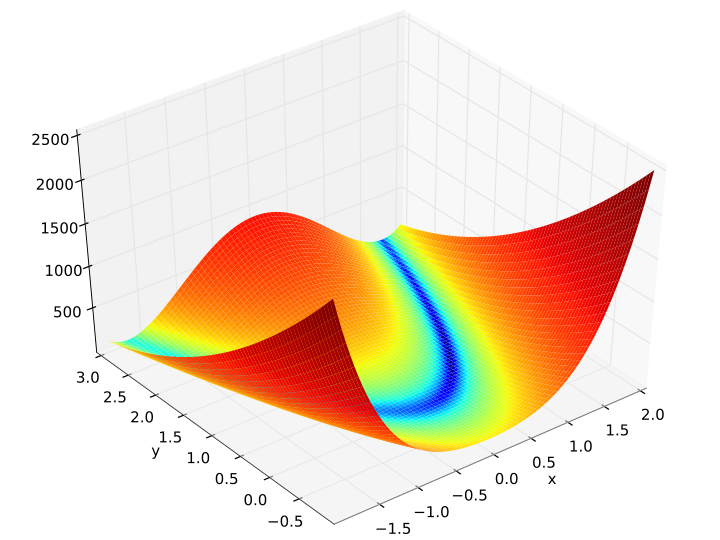
\includegraphics[height=150px]{elias/images/elevation.png}
    \caption{\url{en.wikipedia.org/wiki/rosenbrock_function}}
  \end{figure}
\end{frame}

\begin{frame}{What should be measured?}
  \begin{itemize}
    \item What about the actual behaviour?
    \item Which traits do candidate solutions have?
    \item Categorize according to traits
  \end{itemize}
\end{frame}

%\begin{frame}{What are they good for?}
%  \begin{itemize}
%    \item Cheap evaluation
%  \end{itemize}
%\end{frame}

